\documentclass{article}\usepackage[]{graphicx}\usepackage[]{xcolor}
% maxwidth is the original width if it is less than linewidth
% otherwise use linewidth (to make sure the graphics do not exceed the margin)
\makeatletter
\def\maxwidth{ %
  \ifdim\Gin@nat@width>\linewidth
    \linewidth
  \else
    \Gin@nat@width
  \fi
}
\makeatother

\definecolor{fgcolor}{rgb}{0.345, 0.345, 0.345}
\newcommand{\hlnum}[1]{\textcolor[rgb]{0.686,0.059,0.569}{#1}}%
\newcommand{\hlsng}[1]{\textcolor[rgb]{0.192,0.494,0.8}{#1}}%
\newcommand{\hlcom}[1]{\textcolor[rgb]{0.678,0.584,0.686}{\textit{#1}}}%
\newcommand{\hlopt}[1]{\textcolor[rgb]{0,0,0}{#1}}%
\newcommand{\hldef}[1]{\textcolor[rgb]{0.345,0.345,0.345}{#1}}%
\newcommand{\hlkwa}[1]{\textcolor[rgb]{0.161,0.373,0.58}{\textbf{#1}}}%
\newcommand{\hlkwb}[1]{\textcolor[rgb]{0.69,0.353,0.396}{#1}}%
\newcommand{\hlkwc}[1]{\textcolor[rgb]{0.333,0.667,0.333}{#1}}%
\newcommand{\hlkwd}[1]{\textcolor[rgb]{0.737,0.353,0.396}{\textbf{#1}}}%
\let\hlipl\hlkwb

\usepackage{framed}
\makeatletter
\newenvironment{kframe}{%
 \def\at@end@of@kframe{}%
 \ifinner\ifhmode%
  \def\at@end@of@kframe{\end{minipage}}%
  \begin{minipage}{\columnwidth}%
 \fi\fi%
 \def\FrameCommand##1{\hskip\@totalleftmargin \hskip-\fboxsep
 \colorbox{shadecolor}{##1}\hskip-\fboxsep
     % There is no \\@totalrightmargin, so:
     \hskip-\linewidth \hskip-\@totalleftmargin \hskip\columnwidth}%
 \MakeFramed {\advance\hsize-\width
   \@totalleftmargin\z@ \linewidth\hsize
   \@setminipage}}%
 {\par\unskip\endMakeFramed%
 \at@end@of@kframe}
\makeatother

\definecolor{shadecolor}{rgb}{.97, .97, .97}
\definecolor{messagecolor}{rgb}{0, 0, 0}
\definecolor{warningcolor}{rgb}{1, 0, 1}
\definecolor{errorcolor}{rgb}{1, 0, 0}
\newenvironment{knitrout}{}{} % an empty environment to be redefined in TeX

\usepackage{alltt}
\usepackage{amsmath} %This allows me to use the align functionality.
                     %If you find yourself trying to replicate
                     %something you found online, ensure you're
                     %loading the necessary packages!
\usepackage{amsfonts}%Math font
\usepackage{graphicx}%For including graphics
\usepackage{hyperref}%For Hyperlinks
\usepackage[shortlabels]{enumitem}% For enumerated lists with labels specified
                                  % We had to run tlmgr_install("enumitem") in R
\hypersetup{colorlinks = true,citecolor=black} %set citations to have black (not green) color
\usepackage{natbib}        %For the bibliography
\setlength{\bibsep}{0pt plus 0.3ex}
\bibliographystyle{apalike}%For the bibliography
\usepackage[margin=0.50in]{geometry}
\usepackage{float}
\usepackage{multicol}

%fix for figures
\usepackage{caption}
\newenvironment{Figure}
  {\par\medskip\noindent\minipage{\linewidth}}
  {\endminipage\par\medskip}
\IfFileExists{upquote.sty}{\usepackage{upquote}}{}
\begin{document}

\vspace{-1in}
\title{Lab 8 -- MATH 240 -- Computational Statistics}

\author{
  Andrew Li \\
  Colgate University  \\
  Mathematics Department  \\
  {\tt ali@colgate.edu}
}

\date{}

\maketitle

\begin{multicols}{2}
\begin{abstract}
In this lab, we explored the beta distribution has been explored thoroughly by working with its various properties, probability distributions, and parameters. By changing the parameters, we can evaluate the effects on its statistical values such as mean, variance, skewness, and excess kurtosis. To analyze real world data on global deaths from the World Bank, we made 2 point estimators (Method of Moments and Maximum Likelihood Estimations), which both work well but the \emph{MLE} works slightly better. 

\end{abstract}

\noindent \textbf{Keywords:} point estimations; parameters; probability distributions; 

\section{Introduction}
The beta distribution is a continuous distribution that can be used to model the variability of a random variable $X$ that ranges from $0$ to $1$. It is useful for modeling proportions, probabilities, or rates as its statistical characteristics are versatile enough to assume many different shapes based on its input parameters (Given that $\alpha >$ 0, $\beta >$ 0). 

By exploring its properties, the effects of various inputs can be seen to answer our questions about what the beta distribution is, what it can be used for, what are some of its properties, and what useful inferences can be drawn from simulation and real data analysis. 

The \texttt{R} packages that were used are tidyverse\citep{tidyverse} for data cleaning and plotting, patchwork\citep{patchwork} for combining graphs, e1071\citep{e1071} for calculating properties, xtable\citep{xtable} for table creation, nleqslv\citep{nleqslv} for point estimation calculations, and cumstats\citep{cumstats} for measuring cumulative statistics. 

%\begin{Figure}
%\includegraphics{screenshot}
%\end{Figure}

\section{Density Functions and Parameters}
The beta distribution has a probability density function defined as: 
\[
f(x; \alpha, \beta) = \frac{\Gamma(\alpha + \beta)}{\Gamma\alpha\Gamma\beta} \, x^{\alpha - 1} (1 - x)^{\beta - 1}I(x \in [0,1])
\] 

Knowing that $x$ stays within 0 to 1, we looked at the different cases of \(Beta(\alpha, \beta)\) where \(Beta(2, 5), Beta(5,5), Beta(5, 2), \text{and }Beta(0.5, 0.5)\) and explored their properties. 

The beta distributions for each plot is graphed together in Figure \ref{plot1}.

\section{Properties}
We calculated the population moments using numerical integration shown in Table \ref{table1}.

Since the distribution's shape is affected by its parameters, the population characteristics are also controlled by them. To prove that its possible to approximate what the population distribution might be, we can connect our numerical summaries and graphs to the actual distribution by generating random data and comparing the calculated results against those from the known distribution, shown in Figure \ref{plot2}. The properties of mean, variance, skewness, and excess kurtosis are then compared against those from the population characteristics in Table \ref{table1}.

Then we explored how the law of large numbers is proven to be true as the increasing sample size decreases the variability in the different properties of the data across different samples. This is shown in Figure \ref{plot3} and remains true when we ran random samples and the graphical representations of the properties end up converging towards the population values as sample size increased. 



\begin{table}[H]
\centering
\begin{tabular}{rlrrrr}
  \hline
 & variable & mean & variance & skewness & kurtosis \\ 
  \hline
1 & Beta(0.5,0.5) & 0.50 & 0.12 & 0.00 & -1.50 \\ 
  2 & Beta(2,5) & 0.29 & 0.03 & 0.60 & -0.12 \\ 
  3 & Beta(5,2) & 0.71 & 0.03 & -0.60 & -0.12 \\ 
  4 & Beta(5,5) & 0.50 & 0.02 & 0.00 & -0.46 \\ 
  5 & Sample Beta(0.5,0.5) & 0.52 & 0.12 & -0.11 & 1.55 \\ 
  6 & Sample Beta(2,5) & 0.29 & 0.03 & 0.57 & 2.78 \\ 
  7 & Sample Beta(5,2) & 0.71 & 0.03 & -0.74 & 3.22 \\ 
  8 & Sample Beta(5,5) & 0.50 & 0.02 & 0.06 & 2.54 \\ 
   \hline
\end{tabular} \caption{population moments } \label{table1}
\end{table}

\section{Estimators}
We created a Method of Moments (MOM) point estimator and Maximum Likelihood Estimator (MLE) to calculate the two unknown parameters of $\alpha$ and $\beta$. To use the MOM, we had to find the first two moments of the beta distribution . The first moment is calculated as $\frac{\alpha}{\alpha + \beta}$ while the second is denoted by $\frac {\alpha * (\alpha +1)}{(\alpha + \beta + 1) * (\alpha +\beta)}$. Normally, you can create a symbol of equations and, through substitution, find out what each moment would be using only the sample value for the MOM, and the MLE would have required taking the likelihood of every x and then optimizing the values to find the maximum. We reduced the computations required with \texttt{R}. 






\section{Example}
After running a thousand samples of size 266 with $\alpha$ = 8, $\beta$ = 950 to model the world death data, we were able to compare the accuracy (bias) and variability (precision) of the two point estimators. Looking at the Figure \ref{plot4}, it can be seen that the MLE has less variability because its values doesn't spread as much and has a taller peak. This is further verified when looking at the numerical values in table \ref{table2}, so the MLE is the better point estimator.


% latex table generated in R 4.4.2 by xtable 1.8-4 package
% Thu Apr  3 09:49:34 2025
\begin{table}[H]
\centering
\begingroup\small
\begin{tabular}{rrrlrr}
  \hline
bias & precision & mse & names & actual & estimated \\ 
  \hline
0.08 & 1.83 & 0.55 & moms alpha & 8.00 & 8.08 \\ 
  10.29 & 0.00 & 8288.46 & moms beta & 950.00 & 960.29 \\ 
  0.07 & 2.13 & 0.48 & mles alpha & 8.00 & 8.07 \\ 
  9.11 & 0.00 & 7132.70 & mles beta & 950.00 & 959.11 \\ 
   \hline
\end{tabular}
\endgroup
\caption{Table to compare estimator values} 
\label{table2}
\end{table}


%%%%%%%%%%%%%%%%%%%%%%%%%%%%%%%%%%%%%%%%%%%%%%%%%%%%%%%%%%%%%%%%%%%%%%%%%%%%%%%%
% Bibliography
%%%%%%%%%%%%%%%%%%%%%%%%%%%%%%%%%%%%%%%%%%%%%%%%%%%%%%%%%%%%%%%%%%%%%%%%%%%%%%%%
\vspace{2em}


\begin{tiny}
\bibliography{bib}
\end{tiny}


%%%%%%%%%%%%%%%%%%%%%%%%%%%%%%%%%%%%%%%%%%%%%%%%%%%%%%%%%%%%%%%%%%%%%%%%%%%%%%%%
% Appendix
%%%%%%%%%%%%%%%%%%%%%%%%%%%%%%%%%%%%%%%%%%%%%%%%%%%%%%%%%%%%%%%%%%%%%%%%%%%%%%%%
\newpage
\section{Appendix}


\begin{figure}[H]
\begin{center}
\begin{knitrout}
\definecolor{shadecolor}{rgb}{0.969, 0.969, 0.969}\color{fgcolor}
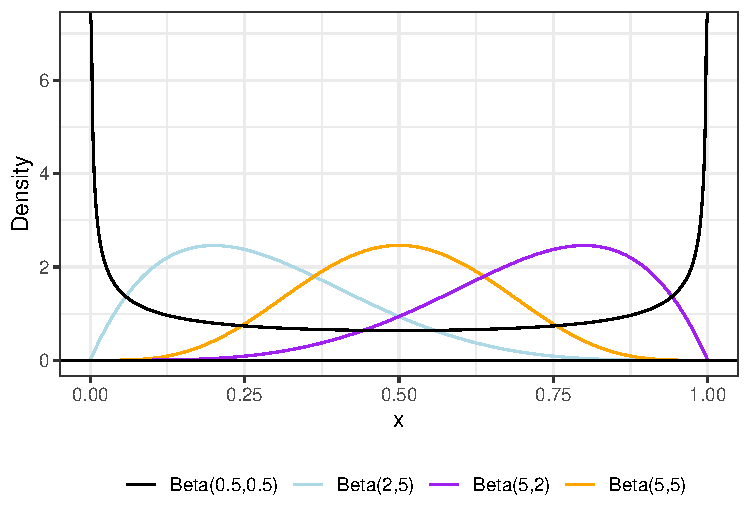
\includegraphics[width=\maxwidth]{figure/unnamed-chunk-5-1} 
\end{knitrout}
\caption{Distributions of different beta plots}
\label{plot1} 
\end{center}
\end{figure}


\begin{figure}[H]
\begin{center}
\begin{knitrout}
\definecolor{shadecolor}{rgb}{0.969, 0.969, 0.969}\color{fgcolor}
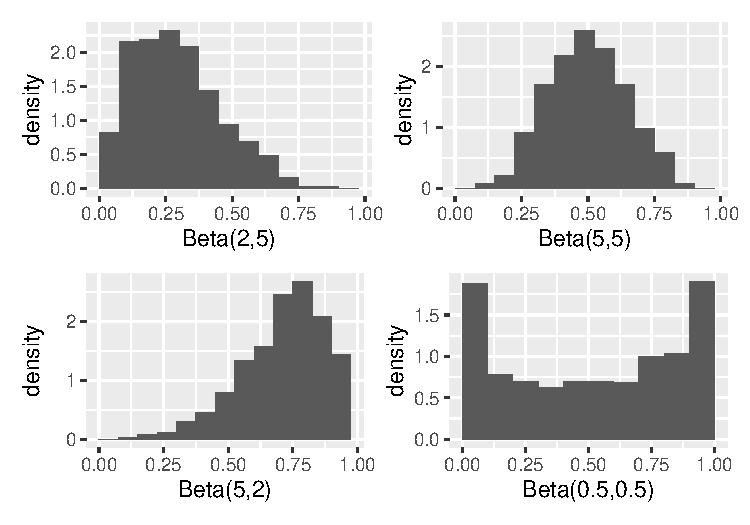
\includegraphics[width=\maxwidth]{figure/unnamed-chunk-6-1} 
\end{knitrout}
\caption{Histograms of densities of beta samples}
\label{plot2} 
\end{center}
\end{figure}



\begin{figure}[H]
\begin{center}
\begin{knitrout}
\definecolor{shadecolor}{rgb}{0.969, 0.969, 0.969}\color{fgcolor}
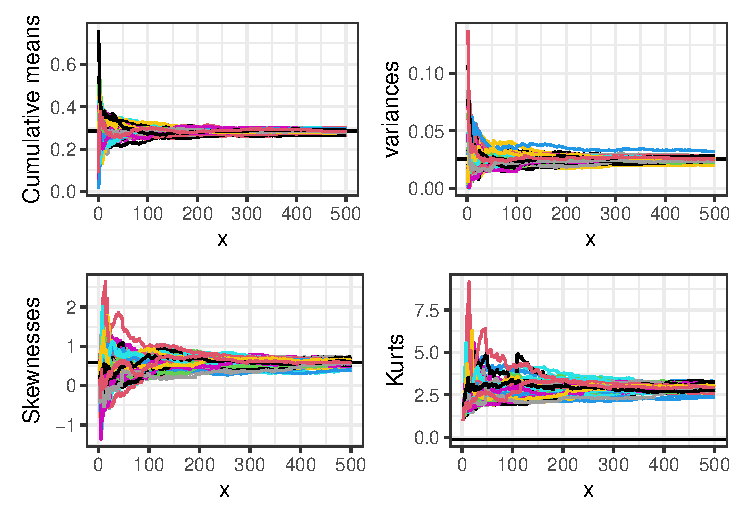
\includegraphics[width=\maxwidth]{figure/unnamed-chunk-7-1} 
\end{knitrout}
\caption{Graphical comparison of random samples to population data}
\label{plot3} 
\end{center}
\end{figure}


\begin{figure}[H]
\begin{center}
\begin{knitrout}
\definecolor{shadecolor}{rgb}{0.969, 0.969, 0.969}\color{fgcolor}
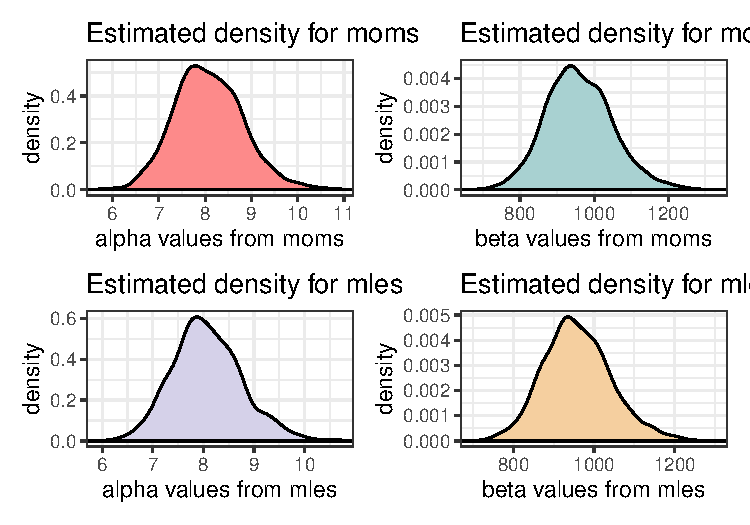
\includegraphics[width=\maxwidth]{figure/unnamed-chunk-8-1} 
\end{knitrout}
\caption{Densities of alpha and beta values from point estimators}
\label{plot4} 
\end{center}
\end{figure}


\end{multicols}
\end{document}
